\begin{minipage}[t]{180mm}
\fcolorbox{black}{white}{
\begin{minipage}[b]{30mm}

\includegraphics[width=0.5\linewidth]{unflogo.pdf}
\end{minipage}
\begin{minipage}[b]{100mm}
\Huge \textbf{UNF NEWZ} \\
\Large -- Søvn og retsstavning er overvurderet! 
\end{minipage}
\begin{minipage}[b]{50mm}
\Large Onsdag 17.07.2015 \\
\normalsize Redigeret i \LaTeX\ af \\ SOM, MGS, MMN, SABH
\end{minipage}
}
\end{minipage}



\begin{minipage}[b]{0.95\linewidth}
\begin{minipage}[t]{0.47\textwidth}
\vspace{3mm}
\section*{Brandbelæring}
Vi er blevet gjort opmærksom på, at den brandbelæring deltagerne modtog søndag ikke var fyldestgørende, så derfor kommer der her en mere udførlig brandbelæring. I tilfælde af mindre brand på instituttet skal Auditorium E forlades gennem nødudgangene og alle skal samle sig på græsplanen. Såfremt branden viser sig at være større, vil også denne plane skulle forlades, og vi samles i stedet på pladsen overfor Statsbiblioteket. I fald af at branden vokser sig større, specielt hvis den skulle gribe over til kemi, er dette sted på randen af Universitetsparken dog lidt for tæt på, og vi vil derfor i stedet samle os på Østbanetorvet, hvilket ved endnu større brande, for eksempel i Fysiks accelerator også gør det lettere at forlade byen ad sø- eller landvejen. Skulle branden skyldes krigeriske handlinger, specielt med fissionsvåben, anbefales det at Jylland forlades omgående, til dette formål er der flere mulige router. Det letteste er måske at tage en båd fra havnen, dette ville dog kræve adgang og tilsvarende færdigheder. Da dette ikke kan forventes af alle deltagere på campen, er en anden mulighed at forlade byen til fods enten mod nord, eventuel for at nå færger til Sverige eller Norge eller mod Syd for at nå den tyske grænse. Eb flugt over land mod vest kan ikke umiddelbart anbefales, da dette kun ville åbne muligheden for at tage færgen fra Esbjerg mod de britiske øer. Skulle vi komme ud for, at der også vil blive anvendt fusionsvåben, anbefaler vi desuden at hele kontinentet forlades. Dette kan klares ved at vandre mod øst, og krydse Uralbjergene, hvilket vil være hård, men give mulighed for en ny tilværsel i Asiens stepper. Desuden kunne det prøves at krydse middelhavet eller atlanten på tømmerflåder eller midnre både, skulle dette overleves ville der være mulighed for en fortsat eksistens i Afrika eller på de amerikanske dobbeltkontinent. På denne tid af året, vil pakisen omkring nordpolen sandsynligvis ikke være stabil nok til at gå til Gørnland eller Canada, så denne route anbefales kun til nøds. Desværre er der en vis risiko for total biologisk uslettelse af alle højere livsformer på jorden, denne kan vi også håndtere, ved ad ovenstående router at bevæge os til Bajkonur (eller til nøds Cape Canaverel) bortføre et rumskib og flytte til ISS eller Månen. Hvis der derimpod er tale om fysisk udslettelse af jordkloden må dette forventes ikke at ære nok, og der tilrådes derfor hurtigst muligt at udvikle den nødvendige teknologi for en etvejsrejse til Mars. Nu burde alle menneskeskabte eventualiteter være afklaret, men vi bør også være forberedt på solens udslettelse da denne ville medføre visse problemer for campens gennemførsel. I dette sammenhæng bør deltagere sende dem selv, helst i frosset tilstand, mod nære stjerner med formodede planeter i håb om at kunne grundlægge en ny civilisation der. Desværre er denne strategi dog indtil videre begrænse på denne galaxis, såfremt hele mælkevejen udslettes ville vi derfor skulle improvisere en effektiv løsning, hvilke de mere intelligente detagere sikkert sagtens kunne klare efter en kop medbragt kaffe eller to. Skulle det komme til universets fulde destruktion, må vi stille større krav til deltagernes selvstændige overlevelsesevner, da dette kræver en duel med penne mod Plato i en velkendt restaurant, i hvilken sejren vil åbne en dør til ideernes verden, og fortsat eksistens i Eulers have med lov til at spise identiteten fra Cayleys træ.


\end{minipage}
\hfill\begin{minipage}[t]{0.47\textwidth}

\vspace{1mm}
\tikzstyle{mybox} = [draw=white, fill=blue!20, very thick,
    rectangle, rounded corners, inner sep=10pt, inner ysep=20pt]
\tikzstyle{fancytitle} =[fill=red, text=white]

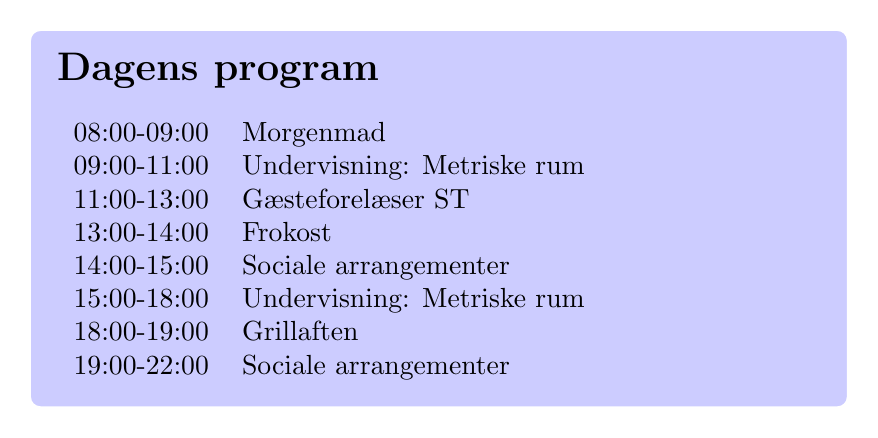
\begin{tikzpicture}
\node [mybox] (box){%
\begin{minipage}{0.80\textwidth}
\vspace{-4mm}\section*{Dagens program}
\begin{tabular}{ll}
08:00-09:00 & Morgenmad \\
09:00-11:00 & Undervisning: Metriske rum \\
11:00-13:00 & Gæsteforelæser ST \\
13:00-14:00 & Frokost \\
14:00-15:00 & Sociale arrangementer \\
15:00-18:00 & Undervisning: Metriske rum \\
18:00-19:00 & Grillaften \\
19:00-22:00 & Sociale arrangementer
\end{tabular}
\vspace{-4mm}
\end{minipage}
};
\end{tikzpicture}%
\vspace{2mm}



\end{minipage}
\end{minipage}
